\documentclass[draft, 10pt]{IEEEtran}

\usepackage{color,soul}
\usepackage{tikz}
\usetikzlibrary{shapes.geometric, arrows, shapes.arrows, decorations.markings, calc}
\usepackage{pgfplots}

\usepackage[english]{babel}
\usepackage{graphicx}
\usepackage{subcaption}
\usepackage{hyperref}
\usepackage{cite}
\usepackage{multirow}

%for flowcharts
\tikzstyle{testing} = [
	thick,
	->,
	>=stealth
]
\tikzstyle{training} = [
	thick, 
	decoration={
		markings,
		mark=at position 1 with {
			\arrow[semithick]{open triangle 60}
		}
	},
	double distance=1.4pt, 
	shorten >= 5.5pt,
	preaction = {decorate},
	postaction = {
		draw,
		line width=1.4pt,
		white,
		shorten >= 4.5pt
	}
]

\tikzstyle{data} = [
	cylinder, 
	shape border rotate=90, 
	draw,
	minimum width=1.5cm, 
	minimum height=1.2cm,
	text centered, 
	draw=black, 
	line width=0.3mm,
	shape aspect=.1
]

\tikzstyle{operation} = [
	rectangle, 
	rounded corners,
	minimum width=2cm, 
	minimum height=1.2cm,
	text centered, 
	draw=black, 
	line width=0.6mm,
]

\tikzstyle{sample} = [
	rectangle, 
	minimum width=1.2cm, 
	minimum height=1.2cm,
	text centered, 
	draw=black,
	line width=0.3mm,
]

\tikzstyle{metric} = [
	diamond, 
	minimum width=1.2cm, 
	minimum height=1.2cm,
	text centered, 
	draw=black,
	line width=0.3mm,
]

\tikzstyle{filter} = [
	trapezium, 
	trapezium left angle=70, 
	trapezium right angle=110, 
	minimum width=1.5cm, 
	minimum height=1cm, 
	text centered, 
	draw=black, 
	line width=0.5mm
]

\begin{document}

\title{\hl{On the use of Generative adversarial neural networks for computing photonic crystal fiber optical properties}}

\author{Aimen Zelaci, Ahmet Yaşlı, Cem Kalyoncu, and Hüseyin Ademgil}

\maketitle
	
\begin{abstract}
Photonic crystal fibers (PCF) for specific applications are designed and optimized by both industry experts and researches. However, the potential number of combinations possible for a single application is very large. This issue combined by the speed of the commonly used Full Vectorial Finite Element Method (FV-FEM) causes the task to take significant amount of time. As stated in the previous works, artificial neural networks (ANN) can predict the result of numerical simulations much faster. However, there are two issues with the methods proposed previously: the required number of samples for training and the generality of these methods. In this paper, we  propose the use of generative adversarial networks (GAN) to augment the real dataset to train an ANN model. Experimental analysis suggest that the proposed combination not only accurately predicts the confinement loss even with limited amount of data but also GAN can be used to improve existing methods in the literature. Finally, it is shown that this system can predict the confinement loss over a range of analytes and wavelengths in a completely new set of geometric configuration and generic enough not to require any additional tuning when used in a new dataset.
\end{abstract}

\section{Introduction}

\hl{Importance of PCF and SPR, written by AY or HA}
	
Machine Learning (ML) techniques are becoming a common tool in many fields, surpassing human performance in many tasks, namely automatic speech recognition, image recognition, natural language processing, drug discovery and toxicology. Additionally, ANN can approximate any function proven by Universality theorem \cite{HORNIK1991251}. This fact propelled researchers to widen the applications of ANN even further, including the study of nanophotonic structures \cite{kiarashinejad2020knowledge}, optimization of photonic crystal nanocavities \cite{asano2018optimization}, and more recently, computing optical properties of a photonic crystal fiber \cite{paper0}.

One of the most difficult challenges that deep learning models face is that they benefit from large amounts of data to train, which may be costly to acquire. One of the solutions to overcome this issue is to artificially expand the original training dataset by the means of generative networks. Introduced by Goodfellow et al., Generative Adversarial Networks (GAN) \cite{goodfellow2014generative}, proved to be successful in data generation \cite{schlegl2017unsupervised, zheng2017unlabeled, frid2018synthetic, tanaka2019data, perez2017effectiveness}.

In this paper, we focus on estimating confinement loss, one of the propagation features of multi-channel Photonic Crystal Fiber (PCF) sensors, using artificial neural networks. Specifically, we have based our system on Surface Plasmon Resonance (SPR). However, in the experiments section we have demonstrated that the designed system is generic enough to apply to multiple PCF designs. The most important contribution of this research is the use of GAN phase, where the available data is expanded to be used in the training phase.


\hl{!! Literature survey !!}

\hl{Use of ANN in PCF}

\hl{SPR in PCF}

This paper is organized as follows. Section \ref{sec:prop} details the use of GAN to generate additional training samples for ANN as well as the proposed neural network architecture. Photonic crystal fiber design that is used for testing is described in details in section \ref{sec:pcf}. Detailed analysis of the experimental results are discussed in section \ref{sec:exp}. Finally, concluding remarks are made in section \ref{sec:conc}.

\section{Proposed method}
\label{sec:prop}

In this section details of the proposed method is discussed. Training of the system contains two phases: a GAN phase and regression training phase. At the start of the training, a GAN is trained to generate additional data by using training samples. These generated samples are filtered to ensure they fall within the applicable range. Original training samples and remaining samples are joined to train a fully-connected feed-forward multi layer perceptron neural network. At the end of the training, the ANN that is trained for the regression task will be used to decide the containment loss  of a set of input parameters. This architecture is illustrated in Figure \ref{fig:overall}. The details of the proposed GAN and ANN architecture is discussed in the following subsections.

\begin{figure}
	\centering
	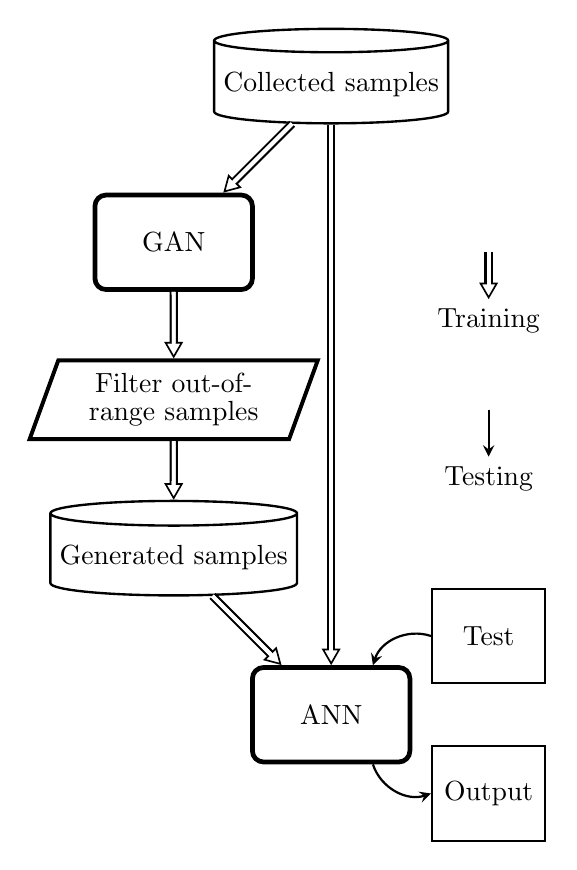
\begin{tikzpicture}[node distance=2cm]
\node (collected) [data] {Collected samples};
\node (GAN) [operation,below of=collected,xshift=-2cm] {GAN};
\node (filter) [filter, below of=GAN, text width=2.4cm] {\baselineskip=10pt Filter out-of-range samples\par};
\node (generated) [data, below of=filter] {Generated samples};
\node (ann) [operation,below of=generated,xshift=2cm] {ANN};
\node (testsample) [sample, right of=generated,xshift=2cm,yshift=-1cm, text width=1.2cm] {\baselineskip=10pt Test\par};
\node (output) [sample, below of=testsample,yshift=-0cm, text width=1.2cm] {\baselineskip=10pt Output\par};

\node (legendtrain) [right of=GAN,xshift=2cm] {};
\node (legendtrainend) [below of=legendtrain,yshift=1cm] {Training};
\node (legendtest) [below of=legendtrainend,yshift=1cm] {};
\node (legendtestend) [below of=legendtest,yshift=1cm] {Testing};


\draw [training] (collected) -- (GAN);
\draw [training] (GAN) -- (filter);
\draw [training] (filter) -- (generated);
\draw [training] (generated) -- (ann);
\draw [training] (collected) -- (ann);
\draw [testing] (testsample.west) to [bend right=45] ($(ann.north east)-(0.5,0)$);
\draw [testing] ($(ann.south east)-(0.5,0)$) to [bend right=45] (output.west);

\draw [training] (legendtrain) -- (legendtrainend);
\draw [testing] (legendtest) -- (legendtestend);

	\end{tikzpicture}
	\caption{System architecture}
	\label{fig:overall}
\end{figure}


\subsection{Generative adversarial network design}
\label{ssec:gan}

Generative adversarial networks are introduced in \cite{goodfellow2014generative}. We have employed GAN to augment the number of samples that are used in training. A GAN is composed of two neural networks: generator and discriminator. The aim of the generator is to transform fully randomized data into data that follows the distribution of the original dataset. Discriminator assesses the performance of the generator and provides feedback for training. Instead of directly training generator, it is trained through this feedback. This paradigm avoids over-fitting the data.

It is possible to use different metrics for training in GAN \hl{[references here]}, for this project we have selected WGAN Wasserstein distance metric. This variant has been proposed by Arjovsky et al in \cite{arjovsky2017wasserstein}. In this system, discriminator is named as critic and it measures the distance between the generated data and the real data. The reason behind choosing WGAN over other methods is to be able to determine a stopping criteria. In a regular GAN system, training is stopped when the generated data is deemed viable by an observer. Since GAN is often used in generation of image, video or audio, using a human in the loop is effective. However, in our problem, it is not viable for a human to judge the generated data. Automating this procedure to remove the human in-the-loop can lead to over or under-fitting, which in turn degrades the performance. WGAN uses an adaptive stopping criteria that does not have the issue mentioned above. Additionally, we have selected to incorporate Gradient penalty to improve WGAN proposed in \cite{gulrajani2017improved}. This improved WGAN system converges in a stable manner without having to fine tune hyper-parameters of the system. The flowchart of this system is given in Figure \ref{fig:gan}.

In this work, both the Critic and the generator are fully connected feed forward MLP models. The details of the networks are given in Table \ref{tbl:anndetails}. The output from this system should be input and output pairs that will be used to train ANN part of the system. In our PCF system we have 6 input parameters and a single output parameter making a total of 7 parameters that will be used in the GAN phase. In Section \ref{sec:exp}, we have experimented using a different PCF system with different inputs, resulting a different number of parameters for the system. The generator is supplied with the same number of parameters as its expected output, that is 7 for our PCF system. These parameters are generated using Gaussian noise and is called latent variable. Once the training phase is complete, the generator and the filter is used to augment the number of training samples that are available for ANN.

Previous works \cite{ravuri2019seeing, shmelkov2018good}, demonstrated that it is possible for random data augmentation to weaken the performance of the model. Hence, it is important to sample the generated data in way to prevent performance degradation \cite{bhattarai2019sampling}. In the proposed system, we have included a filtering step for the generated data. This step uses a simple condition to discard the values that fall out of the desired range, for both the independent variables ($n_{analyte}, \lambda, \Lambda, d1, d2, d3$), and the confinement loss.

\begin{figure}
	\centering
	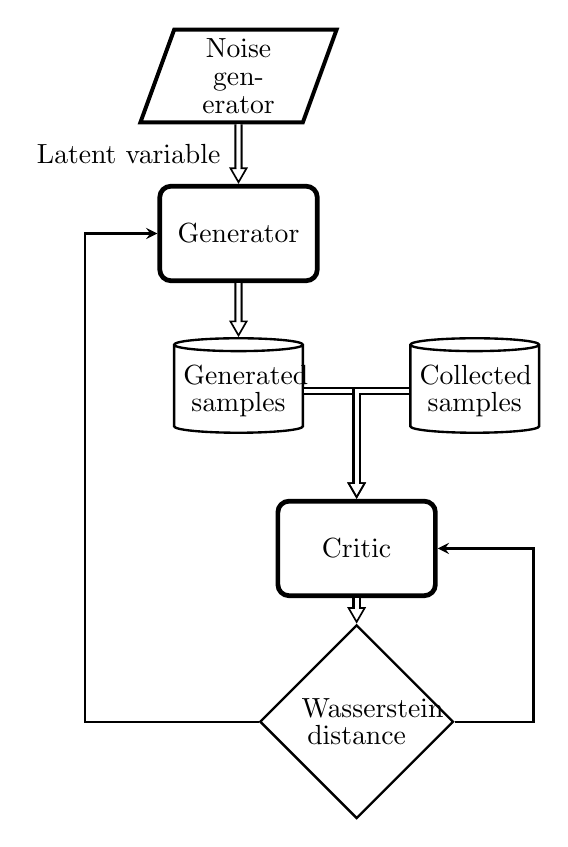
\begin{tikzpicture}[node distance=2cm]
		\node(latent) 	[filter,text width=1.4cm] 		{\baselineskip=10pt Noise generator\par};
		\node(generator)[operation,below of=latent] 	{Generator};
		\node(generated)[data, below of=generator,
						 text width=1.4cm]				{\baselineskip=10pt Generated samples\par};
		\node(collected)[data, right of=generated,
						 xshift=1cm,text width=1.4cm]	{\baselineskip=10pt Collected samples\par};
		\node(critic)	[operation,below of=generated,
						 xshift=1.5cm]					{Critic};
		\node(metric)   [metric,below of=critic,
						 text width=1.4cm, yshift=-.2cm]{\baselineskip=10pt{}Wasserstein distance\par};
		
		\draw [training] (latent) -- (generator) node [pos=.5, left, xshift=-0.1cm] (z) {Latent variable};
		\draw [training] (generator) -- (generated);
		\draw [training] (generated) -| (critic);
		\draw [training] (collected) -| (critic);
		\draw [training] (critic) -- (metric);
		\draw [testing]  (metric.east) - ++(1,0) |-  (critic.east);
		\draw [testing]  (metric.west) - ++(-2.2,0) |-  (generator.west);
	\end{tikzpicture}
	\caption{WGAN training}
	\label{fig:gan}
\end{figure}

\begin{table*}
	\centering
	\caption{Details of ANN models}
	\begin{tabular}{l|l|l|l}
		\textbf{Parameter} & \textbf{Generator} & \textbf{Critic} & \textbf{Regressor} \\\hline
		Hidden layers & 5 & 5 & 6 \\
		Neurons in hidden layers & $ 128 $ & 1024 & 50 \\
		Batch size & 32 & 32 & 48 \\
		Activation function & ReLU & Leaky ReLU & ReLU \\
		Optimizer & Adam \cite{kingma2014adam} & Adam & Adam \\
		Input normalization & None & Z-score (for collected samples) & Z-score \\
		Layer normalization & - & Batch \cite{ioffe2015batch} & Batch \\
		Loss function & Critic(generated) & Critic(generated) - Critic(collected) & MSE \\
	\end{tabular}
	\label{tbl:anndetails}
\end{table*}


\subsection{Artificial neural network design}
\label{ssec:ann}

The ANN model employed in this research is a fully-connected feed-forward Multi Layer Perceptron (MLP) consists of an input layer, an output layer, and 5 hidden layers. The ANN is designed and trained to estimate containment loss in a regression configuration. We have applied $log_{10}$ to confinement loss in order to keep its numeric stability across a wide range. Each hidden layer contains 50 neurons and uses Rectified Linear Unit (ReLU) activation function. Table \ref{tbl:anndetails} summarizes the details of this model.

In our model, we have used mini-batch training with 48 samples as the batch size. In contrast to full-batch training, mini-batch training allows more frequent gradient calculations, improving the stability and reliability of the training \cite{masters2018revisiting, keskar2016large}. The downside of using mini-batches are added computational complexity during training. However, it has no adverse effect on the testing phase.

We have adopted Adam \cite{kingma2014adam} as the optimizer and the mean squared error (MSE) as the loss/cost function. In addition, we use Batch Normalization algorithm \cite{ioffe2015batch} to accelerate training, reduce the effects of initial randomized state and mitigate the problem of internal covariate shift. In proposed system, the ANN is trained using the samples from the original dataset and the augmented samples generated by the GAN phase.


\section{Photonic crystal fiber design}
\label{sec:pcf}

A labelled dataset of only 432 samples was collected in this work, through simulations using FV-FEM. This dataset consists of the wavelength $\lambda$, index of refraction $n_{analyte} $, air-hole to air-hole distance $ \Lambda $, and the air holes radii per ring $d1$, $d2$ and $d3$, taken as our independent variables. The labels are the confinement loss of the PCF. The set consists of nine different configurations of the geometric properties ($ \Lambda $, d1, d2, d3), for each configuration the confinement loss was calculated for three different analytes (Water (n=1.33), Ethanol (n=1.35) and several commercial hydrocarbon mixtures (n=1.36)).

\hl{We will fix the pattern and geometrical shape of the cladding air holes, and vary the wavelength $\lambda$, index of refraction $n_{analyte} $, air-hole to air-hole distance $ \Lambda $, and the air holes radii per ring $d1$, $d2$ and $d3$. Then the results of this study can be carried to different types of SPR-based PCF sensors, using other suitable deep learning approaches such as Recurrent and Convolutional neural networks. }

\hl{PCF design details, written by AY}

\section{Experiments}
\label{sec:exp}

\subsection{Experimental setup}

\def\dszero{PCF}

In order to prove the effectiveness of the proposed setup, we have performed multiple experiments over two datasets. We have built the first dataset that is used in the experiments. This is \hl{an SPR PCF configuration ... and collected using FV-FEM.} Details of this dataset is explained in Section \ref{sec:pcf} and it is referred as SPR dataset. Having nine configurations, we have performed 9-fold testing on this dataset. Each fold tests a single configuration using the other configurations as training data. Slicing the data this way allowed us to guide the network to predict the loss on a completely different configuration. Please note that we have applied $log_{10}$ to confinement loss to scale it.

Additionally, we have used the dataset that has been used in \cite{paper0}. \hl{This dataset contains over 1000 samples. Inputs to this data is .... and outputs are ....} We have only used log of confinement loss as the output. This dataset is referred as \dszero. Details of the datasets that are used in the experiments are given in Table \ref{tbl:dataset}. As a final note, the range and domain of these datasets are different; therefore, all comparisons should be drawn within the same dataset.

We have used mean square error as in the comparisons. All algorithms are implemented using TensorFlow with Keras library in Python and experiments are performed on laptop with Intel i7-5600 CPU and 8GB of RAM. TensorFlow library is set to use only CPU for the experiments.

In the following subsections, we have performed experiments to show the performance of the base ANN system by its own comparing with the state-of-the-art method in the literature \cite{paper0}, improvement gained by employing GAN phase, and finally the computational cost of the overall system compared to the simulator. 5000 training epochs are used for the state-of-the-art method as suggested in the original paper. All numeric comparison results are averaged over multiple executions as listed in Table \ref{tbl:dataset}. Non-averaged data used in charts, such as configuration estimation, are selected from non-extreme cases for the compared methods.

\begin{table}
\centering
\caption{Datasets that are used in experiments}
\begin{tabular}{l|l|l}
	~ & SPR & \dszero \\\hline
	Samples & 432 & 1117\\
	Configurations & 9 & - \\
	Parameters & 6 & 5 \\
	Output & $log_{loss}$ & $log_{loss}$ \\
	Testing & 48 (1 configuration) & 10\% \\
	Testing method & 9-fold & 10-fold \\
\end{tabular}
\label{tbl:dataset}
\end{table}


\subsection{Performance of ANN}

In this set of experiments, we have analyzed the performance of the proposed ANN design. The first experiment involves in training loss over SPR dataset. In this experiment, we have trained ANN model for up to 2000 epochs and reported the training loss in Figure \ref{chart:trainingmse}. We have additionally tested the accuracy with different number of epochs in training. According to this experiment, training our ANN architecture more than 2000 epochs does not yield to any improvement. Therefore, we have set the training epoch limit to 2000 in subsequent experiments. However, this number depends on dataset and at times additional training can improve the result. Additionally, it is clear that the use of augmented samples from the GAN phase reduces the oscillations in the training error.

We have performed experiements comparing the proposed ANN architecture with the state-of-the-art method proposed in \cite{paper0}. Results of this experiment is demonstrated in Figure \ref{chart:perfnoaug}. Please note that in the experiment involving SPR dataset, ANN models are predicting a new configuration and the number of samples available for training is lower. Therefore, they both have higher error rate compared to the \dszero{} dataset. According to Figure \ref{chart:perfnoaug}-c $n_{analyte} = 1.35$ case, the ANN method proposed in \cite{paper0} does not fit to the curve caused by the change in the wavelength. This can be caused by the fact that this method uses full-batch learning \hl{[??]} and therefore under-fits the model. Regardless of this, both models have similar MSE due to the shift in the curve fit. This shift is caused because the network is never exposed to this particular geometric configuration. 


\begin{figure*}
	\begin{subfigure}{.48\textwidth}
	\centering
    \begin{tikzpicture}
		\begin{axis}[
			xlabel=Epochs, 
			ylabel=Training \space MSE,
			width=\textwidth,
			grid=both,
			minor grid style={gray!25},
			major grid style={gray!25},
			ymax=2,
			no marks
		]
		\addplot[line width=1pt,solid,color=blue] %
		table{../../loss_curves_2k/ann_tr_loss_2k_with.txt};
		\end{axis}
	\end{tikzpicture}
	\caption{With augmentation}
	\end{subfigure}	
	\begin{subfigure}{.48\textwidth}
	\centering
	\begin{tikzpicture}
		\begin{axis}[
			xlabel=Epochs, 
			width=\textwidth,
			grid=both,
			minor grid style={gray!25},
			major grid style={gray!25},
			ymax=2,
			no marks
		]
		\addplot[line width=1pt,solid,color=blue] %
		table{../../loss_curves_2k/ann_tr_loss_2k_without.txt};
		\end{axis}
	\end{tikzpicture}
	\caption{Without augmentation}
	\end{subfigure}
		
	\caption{Training MSE of the ANN model with (a) and without (b) GAN phase obtained from SPR dataset}
	\label{chart:trainingmse}
\end{figure*}


\begin{figure*}
\begin{subfigure}{0.48\textwidth}
	\begin{tikzpicture}
		\begin{axis}[
			xlabel=Actual loss in $log(db/cm)$, 
			ylabel=Predicted loss in $log(db/cm)$,
			grid=both,
			minor grid style={gray!25},
			major grid style={gray!25},
			width=\textwidth,
			ymin=5,ymax=7,xmin=5,xmax=7,
			legend pos=south east
		]
			\addplot[
				only marks,
				mark size=2.9pt, mark=o, color=red, fill=red
			] table{../../experiments_spr-pcf/Our_net/Without_augmentation/kfold-predictions-vs-labels/8th/graph_data.txt};
			\addlegendentry{$Proposed$}
			
			\addplot[
				only marks,
				mark size=2.9pt, mark=x, color=green
			] 
			table{../../experiments_spr-pcf/Their_net/without_augmentation/kfold-predictions-vs-labels/5th/graph_data.txt};
			\addlegendentry{\cite{paper0}}
			
			\draw[
				line width=1pt,
				solid,color=blue
			]
			(axis cs:\pgfkeysvalueof{/pgfplots/xmin},\pgfkeysvalueof{/pgfplots/xmin}) -- 
			(axis cs:\pgfkeysvalueof{/pgfplots/xmax},\pgfkeysvalueof{/pgfplots/xmax});
			\addlegendimage{line legend, 
				line width=1pt,
				solid,color=blue}
			\addlegendentry{$Actual$}
			
		\end{axis}
	\end{tikzpicture}
	\caption{SPR dataset}
\end{subfigure}
\begin{subfigure}{0.48\textwidth}
    \begin{tikzpicture}
	\begin{axis}[
		xlabel=Actual loss in $log(db/cm)$, 
		ylabel=Predicted loss in $log(db/cm)$,
		grid=both,
		minor grid style={gray!25},
		major grid style={gray!25},
		width=\textwidth,
		legend pos=south east
	]
		\addplot[
			only marks,
			mark size=2.9pt, mark=o, color=red, fill=red
		] 
		table{../../expirrements_pcf2/Our_net/without_augment/kfold-predictions-vs-labels/2nd/graph_data.txt};
		\addlegendentry{$Proposed$}
		
		\addplot[
		only marks,
		mark size=2.9pt, mark=x, color=green
		] 
		table{../../expirrements_pcf2/Their_net/without_augment/kfold-predictions-vs-labels/2nd/graph_data.txt};
		\addlegendentry{\cite{paper0}}
		
		\draw[
			line width=1pt,
			solid,color=blue
		]
		(axis cs:\pgfkeysvalueof{/pgfplots/xmin},\pgfkeysvalueof{/pgfplots/xmin}) -- 
		(axis cs:\pgfkeysvalueof{/pgfplots/xmax},\pgfkeysvalueof{/pgfplots/xmax});
		\addlegendimage{line legend, 
			line width=1pt,
			solid,color=blue}
		\addlegendentry{$Actual$}
		
		\end{axis}
    \end{tikzpicture}
    \caption{\dszero{} dataset}
\end{subfigure}
\vspace{0.75cm}

\begin{subfigure}{\textwidth}
	\begin{tikzpicture}
	\begin{axis}[
		xlabel=$Wavelength(\lambda) $  $ in $  $ nm $, 
		ylabel=$ Loss $ $ in $ $ Log(db/cm) $,
		grid=both,
		minor grid style={gray!25},
		major grid style={gray!25},
		title={$n_{analyte=1.34}$},
		width=0.48\textwidth,
		legend pos=north west
	]
	\addplot[
		only marks,
		mark size=2.9pt, mark=o, color=red, fill=red
	]
	table[x={wave},y={predicted}]{data/wave_134_our.txt};
	\addlegendentry{$Proposed$}
	
	\addplot[
		only marks,
		mark size=2.9pt, mark=x, color=green
	] 
	table[x={wave},y={predicted}]{data/wave_134_their.txt};
	\addlegendentry{\cite{paper0}}
	
	\addplot[
		color=blue
	] 
	table[x={wave},y={real}]{data/wave_134_our.txt};
	

	\addlegendentry{Actual}
	\end{axis}
	\end{tikzpicture}
	%
	\begin{tikzpicture}
	\begin{axis}[
		xlabel=$Wavelength(\lambda) $  $ in $  $ nm $, 
		ylabel=$~$,
		grid=both,
		minor grid style={gray!25},
		major grid style={gray!25},
		title={$n_{analyte=1.35}$},
		width=0.48\textwidth,
		legend pos=north west
	]
	\addplot[
		only marks,
		mark size=2.9pt, mark=o, color=red, fill=red
	] 
	table[x={wave},y={predicted}]{data/wave_135_our.txt};
	\addlegendentry{$Proposed$}
	            
     \addplot[
		only marks,
		mark size=2.9pt, mark=x, color=green
     ]
	table[x={wave},y={predicted}]{data/wave_135_their.txt};
     \addlegendentry{\cite{paper0}}
	            
	
	\addplot[
		color=blue
	] 
	table[x={wave},y={real}]{data/wave_135_their.txt};
	\addlegendentry{Actual}
	
	\end{axis}
	\end{tikzpicture}
	\caption{Configuration estimation on SPR dataset}
\end{subfigure}
\caption{Testing results without GAN augmentation phase}
\label{chart:perfnoaug}
\end{figure*}


\subsection{Performance boost of GAN}

The first set of experiments performed on GAN phase is the number of the augmented samples. In these experiments we have started augmentation by using 500 samples, increasing it by another 500 per experiment. According to these experiments we have reached the minimum MSE at 1000 samples. Adding further samples reduces the performance and increases the training time. The results of this experiment is demonstrated in Figure \ref{chart:gansamples}. This number may depend on the dataset that is used. However, in our experiments 1000 augmented samples produce good results in both datasets.


\begin{figure}
	\centering
	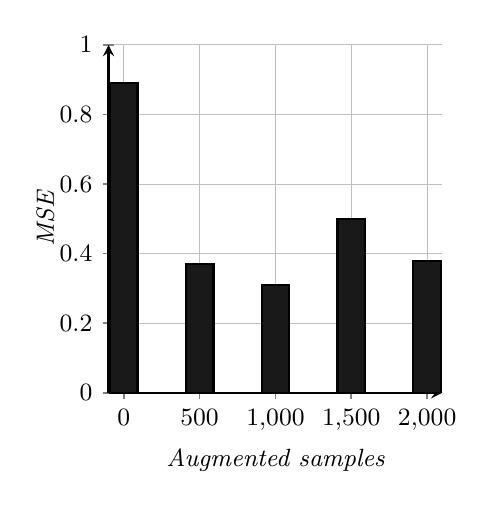
\begin{tikzpicture}[]
	\begin{axis}[
	ybar, axis x line=bottom, xlabel=Augmented samples, 
	xmin=-100,xmax=2100,
	ymin=0,ymax=1,
	width=0.48\textwidth, height=6cm,
	axis y line=left, ylabel=MSE, 
	legend cell align=left,
	legend style={draw=none, at={(0.5,-0.25)},anchor=north,/tikz/every even column/.append style={column sep=1.0cm}}, 
	ylabel near ticks, ylabel shift={-5pt},
	grid = major, legend columns=4
	]
	
	\pgfplotsset{every axis/.append style={font=\small, thick, tick style={semithick}}}
	\pgfplotsset{every axis label/.append style={font=\small\sffamily\it}}
	
	
	\addplot[fill=black!90!white] 
	coordinates {
		(0, 0.89)
		(500, 0.37)
		(1000, 0.31)
		(1500, 0.5)
		(2000, 0.38)
	};
	            
	\end{axis}
	\end{tikzpicture}
	\caption{Effect of increasing augmented samples on MSE.}
	\label{chart:gansamples}
\end{figure}


We have performed experiments to showcase the improvement gained by augmenting training samples using a GAN. In Figure \ref{chart:gan}, the results of these experiments has shown. An additional note to take away from this experiment is that the dataset with the limited number of samples has highest improvement, which is demonstrated in a clearer fashion in Table \ref{tbl:all}.  This is due the fact that the number of training samples in this dataset is insufficient to train the regressor network causing reduced performance.

In Figure \ref{chart:gan}-c, prediction capabilities with and without GAN phase is compared. In the case with $n_{analyte} = 133$, the network without GAN phase has failed to predict the curve correctly. Even though GAN boosted network has predicted the curve lower than it is, the peak is in the correct wavelength, which could help PCF designers to pin-point highest loss.


\begin{figure*}
\begin{subfigure}{0.48\textwidth}
	\begin{tikzpicture}
		\begin{axis}[
			xlabel=Actual loss in $log(db/cm)$, 
			ylabel=Predicted loss in $log(db/cm)$,
			grid=both,
			minor grid style={gray!25},
			major grid style={gray!25},
			width=\textwidth,
			legend pos=south east
		]
			\addplot[
				only marks,
				mark size=2.9pt, mark=o, color=red, fill=red
			] 
			table{../../experiments_spr-pcf/Our_net/Without_augmentation/kfold-predictions-vs-labels/3rd/graph_data.txt};
			\addlegendentry{Without GAN}
			
			\addplot[
				only marks,
				mark size=2.9pt, mark=x, color=green
			]
			table{../../experiments_spr-pcf/Our_net/with_augmentation/kfold-predictions-vs-labels/3rd/graph_data.txt};
			\addlegendentry{With GAN}
			
			\draw[
				line width=1pt,
				solid,color=blue
			]
			(axis cs:\pgfkeysvalueof{/pgfplots/xmin},\pgfkeysvalueof{/pgfplots/xmin}) -- 
			(axis cs:\pgfkeysvalueof{/pgfplots/xmax},\pgfkeysvalueof{/pgfplots/xmax});
			\addlegendimage{line legend, 
				line width=1pt,
				solid,color=blue}
			\addlegendentry{$Actual$}
			\legend{}
		\end{axis}
	\end{tikzpicture}
	\caption{SPR dataset}
\end{subfigure}
\begin{subfigure}{0.48\textwidth}
    \begin{tikzpicture}
	\begin{axis}[
		xlabel=Actual loss in $log(db/cm)$, 
		ylabel=Predicted loss in $log(db/cm)$,
		grid=both,
		minor grid style={gray!25},
		major grid style={gray!25},
		width=\textwidth,
		legend pos=south east
	]
		\addplot[
			only marks,
			mark size=2.9pt, mark=o, color=red, fill=red
		] 
		table{../../expirrements_pcf2/Our_net/without_augment/kfold-predictions-vs-labels/4th/graph_data.txt};
		\addlegendentry{Without GAN}
		
		\addplot[
		only marks,
		mark size=2.9pt, mark=x, color=green
		] 
		table{../../expirrements_pcf2/Our_net/with_augment/kfold-predictions-vs-labels/4th/graph_data.txt};
		\addlegendentry{With GAN}
		
		\draw[
			line width=1pt,
			solid,color=blue
		]
		(axis cs:\pgfkeysvalueof{/pgfplots/xmin},\pgfkeysvalueof{/pgfplots/xmin}) -- 
		(axis cs:\pgfkeysvalueof{/pgfplots/xmax},\pgfkeysvalueof{/pgfplots/xmax});
		\addlegendimage{line legend, 
			line width=1pt,
			solid,color=blue}
		\addlegendentry{$Actual$}
		
		\end{axis}
    \end{tikzpicture}
    \caption{\dszero{} dataset}
\end{subfigure}
\vspace{0.75cm}

\begin{subfigure}{\textwidth}
	\begin{tikzpicture}
	\begin{axis}[
		xlabel=$Wavelength(\lambda) $  $ in $  $ nm $, 
		ylabel=$Loss $ $ in $ $ Log(db/cm) $,
		grid=both,
		minor grid style={gray!25},
		major grid style={gray!25},
		title={$n_{analyte=1.34}$},
		width=0.48\textwidth,
		legend pos=north east,
	]
	\addplot[
		only marks,
		mark size=2.9pt, mark=o, color=red, fill=red
	]
	table[x={wave},y={predicted}]{data/wave_134_our.txt};
	\addlegendentry{Without GAN}
	
	\addplot[
		only marks,
		mark size=2.9pt, mark=x, color=green
	] 
	table[x={wave},y={predicted}]{data/wave_134_aug.txt};
	\addlegendentry{With GAN}
	
	\addplot[
		color=blue
	] 
	table[x={wave},y={real}]{data/wave_134_our.txt};
	\addlegendentry{Actual}\legend{};
	\end{axis}
	\end{tikzpicture}
	%
	\begin{tikzpicture}
	\begin{axis}[
		xlabel=$Wavelength(\lambda) $  $ in $  $ nm $, 
		ylabel=$~$,
		grid=both,
		minor grid style={gray!25},
		major grid style={gray!25},
		title={$n_{analyte=1.33}$},
		width=0.48\textwidth,
		legend pos=north east
	]
	\addplot[
		only marks,
		mark size=2.9pt, mark=o, color=red, fill=red
	] 
	table[x={wave},y={predicted}]{data/wave_133_our.txt};
	\addlegendentry{Without GAN}
	            
     \addplot[
		only marks,
		mark size=2.9pt, mark=x, color=green
     ]
     table[x={wave},y={predicted}]{data/wave_133_aug.txt};
     \addlegendentry{With GAN}
	            
	
	\addplot[
		color=blue
	] 
	table[x={wave},y={real}]{data/wave_133_aug.txt};
	\addlegendentry{Actual}
	\legend{}
	\end{axis}
	\end{tikzpicture}
	\caption{Configuration estimation on SPR dataset}
\end{subfigure}

\label{chart:gan}
\caption{GAN Phase experimental results}
\end{figure*}

We have also applied GAN phase to the network architecture proposed in \cite{paper0}. In this experiment, GAN phase reduced the performance slightly. However, as we have discussed earlier, due to increased number of samples, full batch training strategy is the cause of this. In fact, when we reduce the batch size down to 900 samples, GAN phase starts to improve the score of this architecture.


The final set of experiments shows the stability that GAN phase adds. In Table \ref{tbl:all}, we have listed minimum, maximum, average MSE along with the standard deviation between folds in the testing. It is clear that the GAN phase not only improves the average case but significantly improves the worst case, which is important in a live setting. Even in a dataset with enough examples to train the network (\dszero), using GAN phase reduces the worst case error by 32\%. This added stability can also be observed in Figure \ref{chart:trainingmse}, where the training loss has less fluctuations when the data augmentation is employed.


\begin{table}
\caption{Detailed performance analysis}
\begin{tabular}{l|l|l|l|l|l|l}
	Method & \multicolumn{3}{c|}{SPR} & \multicolumn{3}{c}{\dszero{}} \\\hline
	Dataset & \multicolumn{2}{c|}{Proposed} & \cite{paper0}  & \multicolumn{2}{c|}{Proposed}   & \cite{paper0} \\\hline
	GAN Phase 			& Yes            & No    &  No     &   Yes            & No             & No    \\\hline
	Average   			& \textbf{0.314} & 0.894 & 0.987   &   \textbf{0.134} & 0.156          & 0.167 \\
	Best      			& \textbf{0.006} & 0.042 & 0.047   &   0.095          & \textbf{0.093} & 0.106 \\
	Worst     			& \textbf{1.102} & 6.792 & 5.955   &   \textbf{0.181} & 0.265          & 0.416 \\
	Std. dev.       	& \textbf{0.437} & 2.213 & 1.940   &   \textbf{0.031} & 0.046          & 0.090 \\
\end{tabular}
\label{tbl:all}
\end{table}


\subsection{Computational performance}

In this section we have determined both testing and training time of the proposed system in comparison to the simulation approach. In Table \ref{tbl:timing}, the result of these experiments are published. Training time is total training time while testing is per sample. These tests are performed over SPR dataset. Please note that he training time is considered offline time; i.e., it is the time that will only be used once, before the system is deployed. Once trained, the ANN can work alone without the need for GAN or training again. With this information, it is evident that the ANN based methods are far faster than the simulation approach by several orders of magnitude. Even when training is included, total time spent to calculate the confinement loss will be faster on a GAN boosted ANN compared to FV-FEM simulator after only 5 samples.

The training time difference between ANN systems is caused by the increased depth in the proposed architecture as well as mini-batch training strategy. Training time is dominated by GAN phase; however, this phase does not add any overhead to the testing time. The testing time difference between two networks are caused by the depth of the neural network (6 hidden layers instead of 3). 

\begin{table}
\caption{Execution time of algorithms}
\begin{tabular}{l|l|l}
Method    			  &  Training (s) & Testing (ms) \\\hline
Proposed ANN 		  &  42 & 3.6 \\
Proposed ANN with GAN & 449 & 3.6 \\
GAN phase only        & 370 &  -  \\
\cite{paper0}		  &  20 & 2.7 \\
FV-FEM		   		  &  -  & 106958
\end{tabular}
\label{tbl:timing}
\end{table}

\section{Conclusion}
\label{sec:conc}

In this paper, we have demonstrated that the use of generative adversarial networks can benefit neural networks that are designed to compute photonic crystal fiber optical properties. Additionally, we have also proposed and demonstrated a superior neural network that is both more generic and more powerful to estimate of confinement loss. The GAN phase also reduces the required samples to fully train the ANN, reducing the work necessary to employ the proposed system. The proposed combination is shown to be general enough that even though it is designed for the SPR dataset built for this research; in the experiments, it surpassed the accuracy of the method proposed in \cite{paper0} on the dataset that this state-of-the-art method is optimized on.

Another important aspect in this paper is the experiments performed on a dataset that is designed to test the ability of the neural networks to estimate the properties of a new configuration. For this purpose, we have built a database based on Surface Plasmon Resonance with varying geometric configurations. During testing a new configuration that is not used for the training is used. The proposed ANN, augmented with GAN phase is shown to estimate the new configuration to an acceptable error rate. 

The most important benefit of using machine learning methods instead of simulation is the speed factor. In the experiments it is shown that the machine learning methods works few orders of magnitude faster than the simulation methods. For different types of sensors, Convolutional and Recurrent neural networks can be of great advantage to discover the optimal patterns and geometrical shapes of the cladding air holes. This potential will be explored in a future work.

The code for this work is available at: \url{https://github.com/Aimen-Zelaci/SPRPCF_ANN/}.

\bibliographystyle{IEEEtran}
\bibliography{IEEEabrv,references}	
\end{document}
